% THIS DOCUMENT IS TAILORED TO REQUIREMENTS FOR SCIENTIFIC COMPUTING.  IT SHOULDN'T
% BE USED FOR NON-SCIENTIFIC COMPUTING PROJECTS
\documentclass[12pt]{article}

\usepackage{amsmath, mathtools}
\usepackage{amsfonts}
\usepackage{amssymb}
\usepackage{graphicx}
\usepackage{colortbl}
\usepackage{xr}
\usepackage{hyperref}
\usepackage{longtable}
\usepackage{xfrac}
\usepackage{tabularx}
\usepackage{float}
\usepackage{siunitx}
\usepackage{booktabs}
\usepackage{caption}
\usepackage{pdflscape}
\usepackage{afterpage}
\usepackage{gensymb}
\usepackage{enumitem}
\usepackage[round]{natbib}

%\usepackage{refcheck}

\hypersetup{
    bookmarks=true,         % show bookmarks bar?
      colorlinks=true,       % false: boxed links; true: colored links
    linkcolor=red,          % color of internal links (change box color with linkbordercolor)
    citecolor=green,        % color of links to bibliography
    filecolor=magenta,      % color of file links
    urlcolor=cyan           % color of external links
}

%% Comments

\usepackage{color}

\newif\ifcomments\commentstrue %displays comments
%\newif\ifcomments\commentsfalse %so that comments do not display

\ifcomments
\newcommand{\authornote}[3]{\textcolor{#1}{[#3 ---#2]}}
\newcommand{\todo}[1]{\textcolor{red}{[TODO: #1]}}
\else
\newcommand{\authornote}[3]{}
\newcommand{\todo}[1]{}
\fi

\newcommand{\wss}[1]{\authornote{blue}{SS}{#1}} 
\newcommand{\plt}[1]{\authornote{magenta}{TPLT}{#1}} %For explanation of the template
\newcommand{\an}[1]{\authornote{cyan}{Author}{#1}}

%% Common Parts

\newcommand{\progname}{ProgName} % PUT YOUR PROGRAM NAME HERE
\newcommand{\authname}{Team \#, Team Name
\\ Student 1 name
\\ Student 2 name
\\ Student 3 name
\\ Student 4 name} % AUTHOR NAMES                  

\usepackage{hyperref}
    \hypersetup{colorlinks=true, linkcolor=blue, citecolor=blue, filecolor=blue,
                urlcolor=blue, unicode=false}
    \urlstyle{same}
                                


% For easy change of table widths
\newcommand{\colZwidth}{1.0\textwidth}
\newcommand{\colAwidth}{0.13\textwidth}
\newcommand{\colBwidth}{0.82\textwidth}
\newcommand{\colCwidth}{0.1\textwidth}
\newcommand{\colDwidth}{0.05\textwidth}
\newcommand{\colEwidth}{0.8\textwidth}
\newcommand{\colFwidth}{0.17\textwidth}
\newcommand{\colGwidth}{0.5\textwidth}
\newcommand{\colHwidth}{0.28\textwidth}

% Used so that cross-references have a meaningful prefix
\newcounter{defnum} %Definition Number
\newcommand{\dthedefnum}{GD\thedefnum}
\newcommand{\dref}[1]{GD\ref{#1}}
\newcounter{datadefnum} %Datadefinition Number
\newcommand{\ddthedatadefnum}{DD\thedatadefnum}
\newcommand{\ddref}[1]{DD\ref{#1}}
\newcounter{theorynum} %Theory Number
\newcommand{\tthetheorynum}{TM\thetheorynum}
\newcommand{\tref}[1]{TM\ref{#1}}
\newcounter{tablenum} %Table Number
\newcommand{\tbthetablenum}{TB\thetablenum}
\newcommand{\tbref}[1]{TB\ref{#1}}
\newcounter{assumpnum} %Assumption Number
\newcommand{\atheassumpnum}{A\theassumpnum}
\newcommand{\aref}[1]{A\ref{#1}}
\newcounter{goalnum} %Goal Number
\newcommand{\gthegoalnum}{GS\thegoalnum}
\newcommand{\gsref}[1]{GS\ref{#1}}
\newcounter{instnum} %Instance Number
\newcommand{\itheinstnum}{IM\theinstnum}
\newcommand{\iref}[1]{IM\ref{#1}}
\newcounter{reqnum} %Requirement Number
\newcommand{\rthereqnum}{R\thereqnum}
\newcommand{\rref}[1]{R\ref{#1}}
\newcounter{nfrnum} %NFR Number
\newcommand{\rthenfrnum}{NFR\thenfrnum}
\newcommand{\nfrref}[1]{NFR\ref{#1}}
\newcounter{lcnum} %Likely change number
\newcommand{\lthelcnum}{LC\thelcnum}
\newcommand{\lcref}[1]{LC\ref{#1}}
\newcounter{refnum} %Reference Number
\newcommand{\retherefnum}{REF\therefnum}
\newcommand{\reref}[1]{\ref{#1}}
\newcounter{ulcnum} %Unlike likely change number
\newcommand{\ltheulcnum}{ULC\theulcnum}
\newcommand{\ulcref}[1]{ULC\ref{#1}}

\usepackage{fullpage}

\newcommand{\deftheory}[9][None]
{
\newpage
\noindent \rule{\textwidth}{0.5mm}

\paragraph{RefName: } \textbf{#2} \phantomsection 
\label{#2}

\paragraph{Label:} #3

\noindent \rule{\textwidth}{0.5mm}

\paragraph{Equation:}

#4

\paragraph{Description:}

#5

\paragraph{Notes:}

#6

\paragraph{Source:}

#7

\paragraph{Ref.\ By:}

#8

\paragraph{Preconditions for \hyperref[#2]{#2}:}
\label{#2_precond}

#1

\noindent \rule{\textwidth}{0.5mm}

}

\begin{document}

\title{Software Requirements Specification for Bridge Corrosion: A Chloride Exposure Prediction Model} 
\author{Cynthia Liu}
\date{\today}
	
\maketitle

~\newpage

\pagenumbering{roman}

\tableofcontents

~\newpage

\section*{Revision History}

\begin{tabularx}{\textwidth}{p{3cm}p{2cm}X}
\toprule {\bf Date} & {\bf Version} & {\bf Notes}\\
\midrule
Jan 27, 2024 & 1.0 & Initial release\\
\bottomrule
\end{tabularx}

~\newpage

\section{Reference Material}

This section records information for easy reference.

\subsection{Table of Units}

Throughout this document SI (Syst\`{e}me International d'Unit\'{e}s) is employed
as the unit system.  In addition to the basic units, several derived units are
used as described below.  For each unit, the symbol is given followed by a
description of the unit and the SI name.
~\newline

\renewcommand{\arraystretch}{1.2}
%\begin{table}[ht]
  \noindent \begin{tabular}{l l l} 
    \toprule		
    \textbf{symbol} & \textbf{unit} & \textbf{SI}\\
    \midrule 

    \si{\metre} & length & metre\\
    \si{\kilogram} & mass & kilogram\\
    \si{\second} & time & second\\

    \bottomrule
  \end{tabular}
  %	\caption{Provide a caption}
%\end{table}

\subsection{Table of Symbols}

The table that follows summarizes the symbols used in this document along with
their units.  The choice of symbols was made to be consistent with the heat
transfer literature and with existing documentation for solar water heating
systems.  The symbols are listed in alphabetical order.

\break
\break

\renewcommand{\arraystretch}{1.2}
%\noindent \begin{tabularx}{1.0\textwidth}{l l X}
\noindent \begin{longtable*}{l l p{12cm}} \toprule
\textbf{symbol} & \textbf{unit} & \textbf{description}\\
\midrule 
$a_{splash}$ & $kg/m^3$ & maximum deposition rate occur from splash\\
$a_{spray}$ & $kg/m^3$ & maximum deposition rate occur from spray\\
$a_{air}$ & $kg/m^3$ & maximum deposition rate\\
$b_{splash}$ & N/A & splash emission rate coefficient\\
$b_{spray}$ & N/A & spray emission rate coefficient\\
$C_s$ & $kg/m^3/vehicle$ & chloride on the bridge substructure\\
$C_{s_{air}}$ & $kg/m^3/vehicle$ & chloride sprayed and splashed per unit air volume per vehicle\\
$\delta_{salt}$ & $N/A$ & ratio of salt over water per unit area of road\\
$d$ & $m$ & distance between road edge and nearby bridge structure\\
$h_{app}$ & $m$ & daily water film thickness on the road\\
$h_{film}$ & $m$ & depth of the water film picked up in each rotation\\
$h_{total}$ & $m$ & water equivalent of snowfall\\
$I$ & $m/h$ & rainfall intensity\\
$K$ & $N/A$ & ratio of the tire width that is not a groove to the tire width\\
$L$ & $m$ & drainage length\\
$M_{app}$ & $kg/m^2$ & deicing salts quantity applied per day\\
$M_{total}$ & $kg/m^2$ & total amount of deicing salts quantity over winter\\
$MR_{BW}$ & $kg/s$ & MFR displaced by a single tire due to bow\\
$MR_{CA}$ & $kg/s$ & MFR displaced by a single tire due to capillary adhesion\\
$MR_{SW}$ & $kg/s$ & MFR displaced by a single tire due to side waves\\
$MR_{TP}$ & $kg/s$ & MFR displaced by a single tire due to tread pickup\\
$MR_{W}$ & $kg/s$ & general MFR displaced by a single tire due to capillary adhesion\\
$N_{lane}$ & lane & number of lanes\\
$\rho_{water}$ & $kg/m^{3}$ & density of water\\
$SD_{BW}$ & $kg/m^{3}/vehicle$ & spray density by a single tire due to bow\\
$SD_{CA}$ & $kg/m^{3}/vehicle$ & spray density by a single tire due to capillary adhesion\\
$SD_{SW}$ & $kg/m^{3}/vehicle$ & spray density by a single tire due to side waves\\
$SD_{TP}$ & $kg/m^{3}/vehicle$ & spray density by a single tire due to tread pickup\\
$SD_{total}$ & $kg/m^{3}/vehicle$ & spray density kicked up by each passing truck\\
$SD_{total~cl}$ & $kg/m^3/vehicle$ & mass of chloride ions per unit air volume\\
$S$ & $N/A$ & slope as a ratio\\
$T$ & $mm$ & profile depth\\
$t_1$ & days & number of days with snowfall\\
$t_2$ & days & number of days with snow melting\\
$t_{snow}$ & days & number of days with snow\\
$V$ & $m/s$ & truck speed\\
$V_{salt}$ & $tonnes/cm/km$ & normalized salt application rate\\
$V_{speed}$ & $km/h$ & heavy vehicle speed\\
$V'$ & $miles/h$ & heavy vehicle speed\\
$W_{lane}$ & $m$ & lane width\\
$WD$ & $m$ & water depth/thickness\\
$x$ & $m$ & distance between road and object surface\\
$\Theta$ & $N/A$ & ratio of chloride ions sprayed and splashed by trucks over those by light duty vehicles\\
$\theta_{chloride}$ & $N/A$ & molar mass ratio of chloride ions over deicing salts\\
\bottomrule
\end{longtable*}
\subsection{Abbreviations and Acronyms}

\renewcommand{\arraystretch}{1.2}
\begin{tabular}{l l} 
  \toprule		
  \textbf{symbol} & \textbf{description}\\
  \midrule 
  A & Assumption\\
  DD & Data Definition\\
  GD & General Definition\\
  GS & Goal Statement\\
  IM & Instance Model\\
  LC & Likely Change\\
  PS & Physical System Description\\
  R & Requirement\\
  SRS & Software Requirements Specification\\
  BS & Bridge Corrosion\\
  TM & Theoretical Model\\
  NaCl & Sodium Chloride, the main component of deicing salts \\
  CA & Capillary Adhesion \\
  TP & Tread Pickup\\
  BW & Bow Waves\\
  SW & Side Waves\\
  MFR & Mass Flow Rate\\
  ADT & Average Daily Traffic\\
  AADT & Annual Average Daily Traffic\\
  AADTT & Annual Average Daily Truck Traffic \\
  \bottomrule
\end{tabular}\\

\subsection{Mathematical Notation}
\renewcommand{\arraystretch}{1.2}
\begin{tabular}{l l} 
  \toprule		
  \textbf{symbol} & \textbf{description}\\
  \midrule 
  $\mathbb{R}$ & Real number \\
  \{$\mathbb{R}$\} & a set of real number\\
  \bottomrule
\end{tabular}\\

\newpage

\pagenumbering{arabic}

\section{Introduction}
In Ontario, most of the bridges in highway are made of reinforced concrete (RC) decks. However, the bridges may face the chloride-induced corrosion which damage its surface. There are many elements influencing this situation, one of the most important one is the deicing salts. The primary used is sodium chloride (rock salt),when they melt the snow and in contact with water, they could have a chemical reaction and release the chloride ions. Those chloride could penetrate the concrete and induce corrosion in the reinforcing steel, then damage the bridges’ structure and capacity. \\
There is a tight connection between chloride exposure, weather conditions and traffic flow. Specifically, the amount of deicing salts applied on the road surface greatly depends on the amount of snowfall, and the amount of water and dissolved chloride ions that end up on nearby objects depends on the traffic patterns. This section outlines the document's purpose, delineates its scope of requirements, describes the intended audience's characteristics, and provides an overview of the document's organization.

\subsection{Purpose of Document}
This document details the requirements of the software Bridge Corrosion. The
responsibilities of the user and software are laid out and the requirements that the software must satisfy are explicitly detailed. This document provides the software requirements specification (SRS) for a project to investigate how the climate and traffic could have impact on the corrosion-induced damage for the reinforced concrete, or to be more specific, how they influence the chloride exposure. 

\subsection{Scope of Requirements} 
The entire document is written as the chloride is the main source of corrosion damage to the reinforced concrete, and chloride ions are transported from the road to the exterior surface of bridge substructures through vehicle spray and splash mechanisms. Another scope of the document is the factors that affect bridge corrosion is limit to chloride levels, climatic conditions, and traffic patterns.

\subsection{Characteristics of Intended Reader} \label{sec_IntendedReader}
Readers of this documentation are expected to have a understanding of high school mathematics and chemistry, and the ability to comprehend basic results generated through computational fluid dynamics. The users of Bridge Corrosion may exhibit diverse levels of expertise, as further detailed in Section \ref{SecUserCharacteristics}.

\subsection{Organization of Document}
The organization of this document follows the template for an SRS for scientific computing software proposed by Smith et al. [\reref{ref1}, \reref{ref2}, \reref{ref3}]. Starting with the reference material including units, symbols and abbreviations, this document next introduce the system that we are going to build from general to specific, including the problem, goal, assumptions, theoretical model and instance models. It also talks about the functional and nonfunctional requirements for this project, which could be referred to in process of development.

\section{General System Description}

This section provides general information about the system.  It identifies the
interfaces between the system and its environment, describes the user
characteristics and lists the system constraints.  
\subsection{System Context}
Figure 1 shows the system context of the software. The user should input a coordinates to the software, and the software will return the predicted chloride exposure over time to the user. The user and the software also assume the following responsibilities.

\begin{figure}[h!]
\begin{center}
 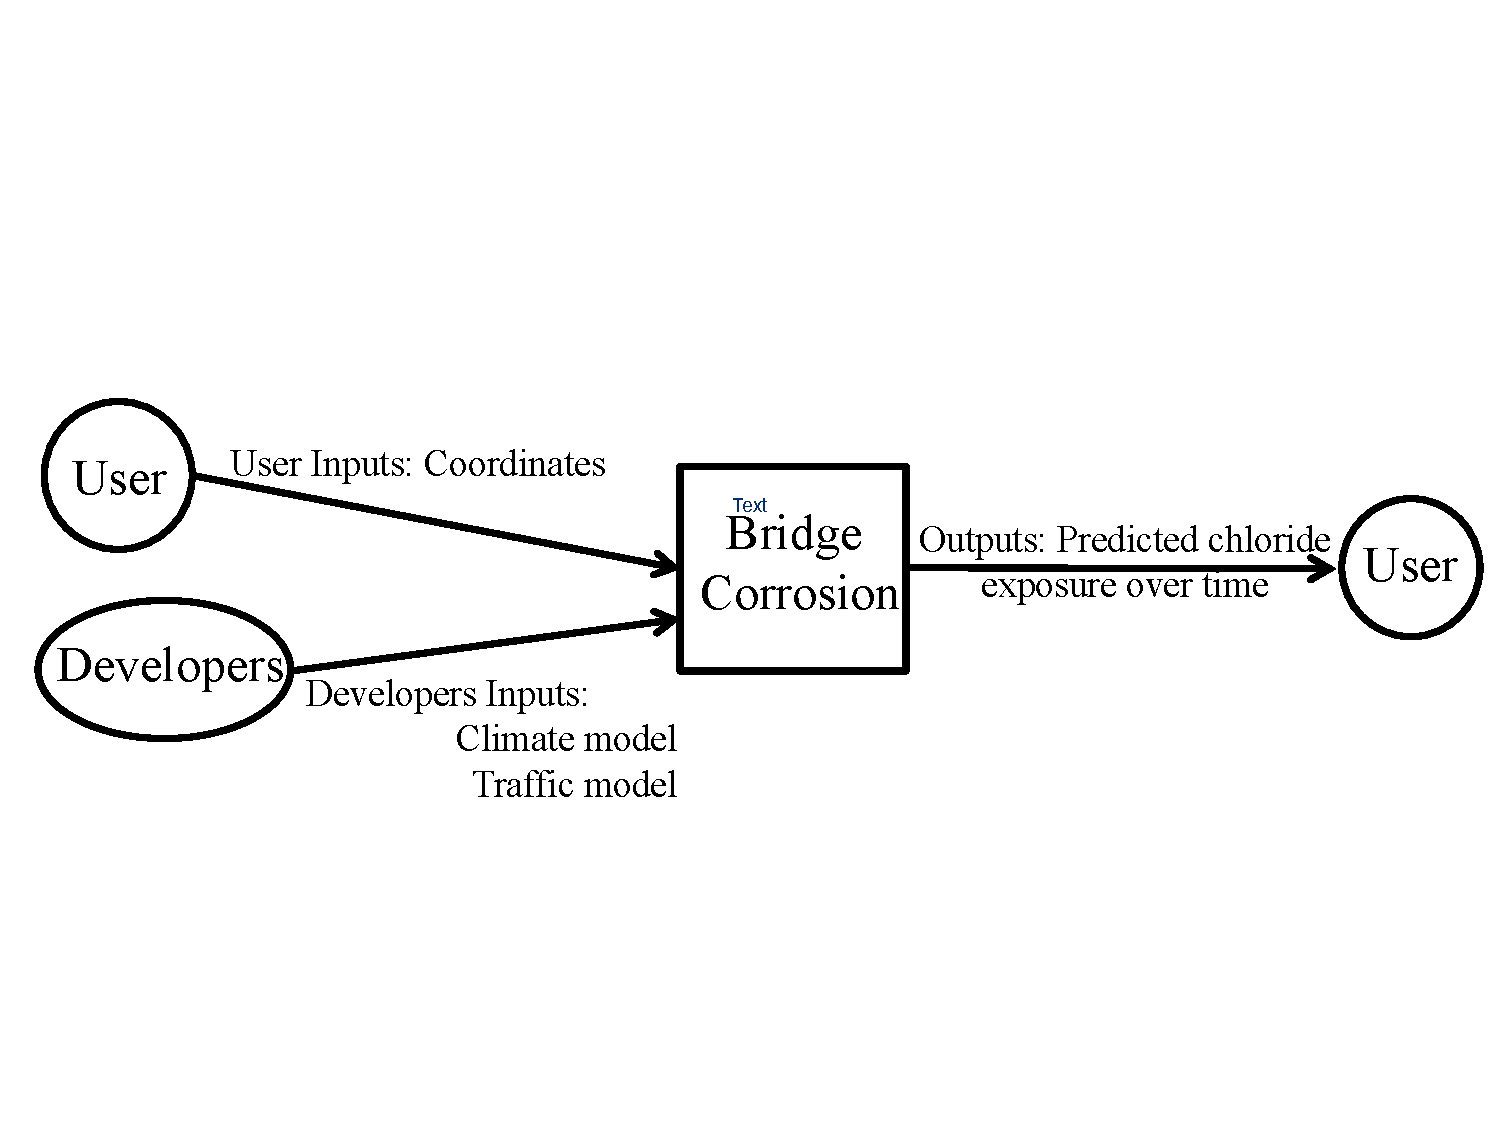
\includegraphics[width=0.8\textwidth]{SystemContextFigure}
\caption{System Context}
\label{Fig_SystemContext} 
\end{center}
\end{figure}

\begin{itemize}
\item User Responsibilities:
\begin{itemize}
\item Provide valid coordinates to the software.
\end{itemize}
\item Bridge Corrosion Responsibilities:
\begin{itemize}
\item Build a database storing the chloride exposure data for every 25 km over time.
\item Search and return the chloride exposure trend at given input coordinate.
\item Provide visualization of the output.
\end{itemize}
\end{itemize}

\subsection{User Characteristics} \label{SecUserCharacteristics}
The end user of Bridge Corrosion should have the basic understanding of geographic coordinates. Additionally, users may benefit from some knowledge of bridge construction or civil engineering principles to better understand the context and implications of the predicted chloride exposure.


\subsection{System Constraints}
 The software must be able to provide output for coordinates inside Ontario. 
  
\section{Specific System Description}

This section first presents the problem description, which gives a high-level
view of the problem to be solved.  This is followed by the solution characteristics
specification, which presents the assumptions, theories, definitions and finally
the instance models.  

\subsection{Problem Description} \label{Sec_pd}
This project is intended to investigate how climate, traffic might impact corrosion-induced damage for reinforced concrete bridges by influencing the chloride exposure.

\subsubsection{Terminology and  Definitions}
This subsection provides a list of terms that are used in the subsequent
sections and their meaning, with the purpose of reducing ambiguity and making it
easier to correctly understand the requirements:

\begin{itemize}
\item Mass flow rate: The amount of water displaced by a single tire.
\item Spray density: The water concentration (mass of water per unit air volume) in the environment.
\item Airborne deposition: The process of particles moving from the atmosphere to the earth's surface.
\item Deposition rate: The rate at which a substance is deposited onto a surface over a specific period of time.

\end{itemize}

\subsubsection{Physical System Description} \label{sec_phySystDescrip}


The key physical system of Bridge Corrosion, as shown in Figure \ref{4mechanism}, simulate the situation that a vehicle spray and splash the water, it includes the following elements:

\begin{itemize}

\item[PS1:] Capillary adhesion: The absorption of water (present on the road surface) by the tires through surface tension.

\item[PS2:] Tread pickup: Water within the grooves of a tire being sprayed and splashed behind the tire by turbulent flow in the grooves.

\item[PS3:] Bow wave: Water sent towards the front of the tire because of the physical displacement of water from the road surface due to the vehicle tires.

\item[PS4:] Side wave: Water sent in the direction perpendicular to the traffic because of the physical displacement of water from the road surface due to the vehicle tires.

\end{itemize}


\begin{figure}[h!]
\begin{center}
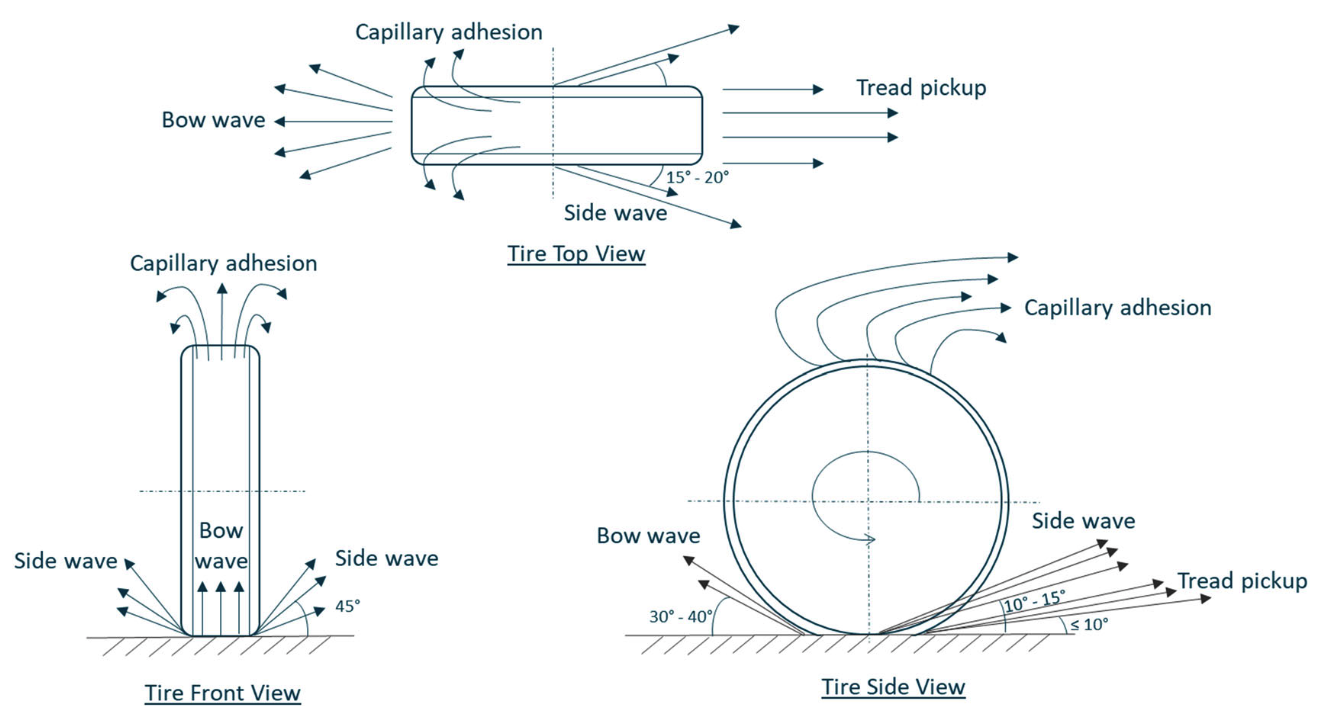
\includegraphics[width=0.9\textwidth]{phymodel}
\caption{\label{4mechanism} Mechanisms of vehicle spray and splash}

\end{center}
\end{figure}

% \begin{figure}[h!]
% \begin{center}
% %\rotatebox{-90}
% {
%  \includegraphics[width=0.5\textwidth]{<FigureName>}
% }
% \caption{\label{<Label>} <Caption>}
% \end{center}
% \end{figure}

\newpage
\subsubsection{Goal Statements}

\noindent Given the salt application data, climate data and traffic data across different regions and time period , the goal statements are:

\begin{itemize}

\item[GS\refstepcounter{goalnum}\thegoalnum \label{G_ChlorideExposurePrediction}:] Predict the chloride exposure for bridges in Ontario over time.

\item[GS\refstepcounter{goalnum}\thegoalnum \label{G_ExtractData}:] Allow user to input coordinate and return the prediction for the nearest bridge.

\end{itemize}

\subsection{Solution Characteristics Specification}

\begin{figure}[H]
  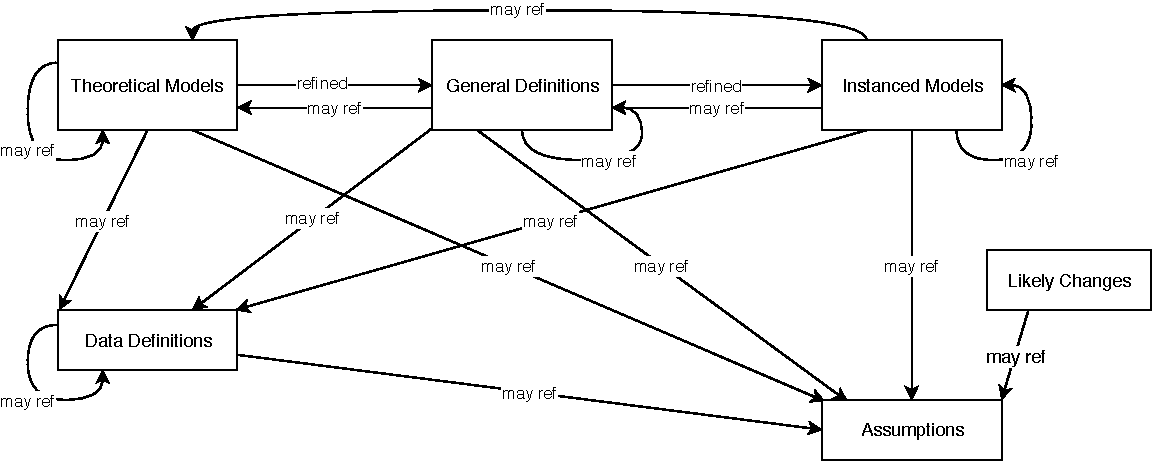
\includegraphics[scale=0.9]{RelationsBetweenTM_GD_IM_DD_A.pdf}
\end{figure}

The instance models that govern this project are presented in
Subsection~\ref{sec_instance}.  The information to understand the meaning of the
instance models and their derivation is also presented, so that the instance
models can be verified.

\subsubsection{Types}

Input:
\begin{itemize}
\item longitude = $\mathbb{R}$
\item latitude = $\mathbb{R}$

\end{itemize}
Output:
\begin{itemize}
\item predictedChlorideExposure = \{$\mathbb{R}$\}
\end{itemize}


\subsection{Scope Decisions}
The surface chloride exposure data is in a 25-km grid resolution. This is because the climate data extracted from the CanRCM4 model (Scinocca et al. 2016) at a resolution of 25 × 25 km.

% \plt{This section is optional.}
\subsection{Modelling Decisions}

\subsubsection{Assumptions} \label{sec_assumpt}

This section simplifies the original problem and helps in developing the
theoretical model by filling in the missing information for the physical system.
The numbers given in the square brackets refer to the theoretical model [TM],
general definition [GD], data definition [DD], instance model [IM], or likely
change [LC], in which the respective assumption is used.

\begin{itemize}

\item[A\refstepcounter{assumpnum}\theassumpnum \label{A_deicingSalts}:] All the deicing salts are applied on days with snowfall. (RefBy: \tref{T_CSASG}, \dref{D_CSAS}, \ddref{DD_DSQ}, \ddref{DD_DWFT})


\item[A\refstepcounter{assumpnum}\theassumpnum \label{A_laneWidth}:] The lane width for all the roads are the same. (RefBy: \ddref{DD_DSQ}, \lcref{LC_laneWidth})

\item[A\refstepcounter{assumpnum}\theassumpnum \label{A_NaCl}:] The main component of deicing salt is NaCl. (RefBy: \ddref{DD_RCL}, \ddref{DD_SDTCL})

\item[A\refstepcounter{assumpnum}\theassumpnum \label{A_AADT}:] Same class of the road over which the bridge spans has the same AADT. (RefBy: \dref{D_CSAS}, \lcref{LC_AADT})

\end{itemize}

\subsubsection{Theoretical Models}\label{sec_theoretical}
This section focuses on the general equations and laws the project is based on. 
\newline
\noindent

%TM1
\noindent
\begin{minipage}{\textwidth}
\renewcommand*{\arraystretch}{1.5}
\begin{tabular}{| p{\colAwidth} | p{\colBwidth}|}
\hline
\rowcolor[gray]{0.9}
Number& TM\refstepcounter{theorynum}\thetheorynum \label{T_WFT}\\
\hline
Label &\bf Water film thickness\\
\hline
% Units&$MLt^{-3}T^0$\\
% \hline
SI Units&\si{m}\\
\hline
Equation& $WD = 6 \times 10^{-4} \cdot T^{0.09} (L \cdot I)^{0.6} \cdot S^{-0.33} $\\
\hline
Description & 
The above equation compute the water film thickness based on the rainfall intensity and pavement surface properties.
\begin{itemize}

\item $WD$ is the water depth. ($m$)

\item $T$ is the texture. ($mm$)

\item $L$ is the drainage length. ($m$)

\item $I$ is the rainfall intensity. ($m/h$)

\item $S$ is the slope. (ratio)


\end{itemize}

\\
\hline
  Source & [\reref{ref5}] \\
  \hline
  Ref.\ By & \tref{T_MFRG} \\
  \hline
\end{tabular}

\end{minipage}\\


%TM2
\noindent
\begin{minipage}{\textwidth}
\renewcommand*{\arraystretch}{1.5}
\begin{tabular}{| p{\colAwidth} | p{\colBwidth}|}
\hline
\rowcolor[gray]{0.9}
Number& TM\refstepcounter{theorynum}\thetheorynum \label{T_MFRG}\\
\hline
Label &\bf Max flow rate general \\
\hline
% Units&$MLt^{-3}T^0$\\
% \hline
SI Units&\si{kg\per s}\\
\hline
Equation& $MR_W = V \cdot b \cdot WD \cdot \rho_{water} $\\

\hline
Description & 
The above equation is the general equation for mass flow rate, which is the maximum amount of water available for splash and spray.
\begin{itemize}

\item $V$ is the truck speed. ($m/s$)

\item $b$ is the tire width. ($m$)

\item $WD$ is the water depth/thickness. ($m$)

\item $\rho_{water}$ is the density of water. ($kg/m^{3}$)

\end{itemize}


\\
\hline
  Source & [\reref{ref5}] \\
  \hline
  Ref.\ By & \dref{D_MFR}\\ 
  \hline
  Use\ & \tref{T_WFT}\\
  \hline
\end{tabular}

\end{minipage}\\

%TM3
\noindent
\begin{minipage}{\textwidth}
\renewcommand*{\arraystretch}{1.5}
\begin{tabular}{| p{\colAwidth} | p{\colBwidth}|}
  \hline
  \rowcolor[gray]{0.9}
  Number& TM\refstepcounter{theorynum}\thetheorynum \label{T_CSASG}\\
  \hline
  Label& \bf Chloride sprayed and splashed \\
\hline
% Units&$MLt^{-3}T^0$\\
% \hline
SI Units&\si{kg\per\metre^3\per vehicle} \\
\hline
Equation & $C_{{s}_{air}} = (SD_{total~cl} \times \frac{1}{\Theta} \times \frac{ADT-N}{N_{lane}}+ SD_{total~cl} \times \frac{N}{N_{lane}}) \times t_{snow}$ \\
  \hline
  Description& The above equation computes the mass of chloride ions per unit air volume sprayed and splashed by all the vehicles passing near the bridge pier every winter, accounting for all the days with snow in a typical winter season.
  
\begin{itemize}

\item $SD_{total~cl}$ is the mass of chloride ions per unit air volume. ($kg/m^3/vehicle$)

\item $\Theta$ is the ratio of chloride ions sprayed and splashed by trucks to light-duty vehicles. (ratio)

\item $ADT$ is the average daily traffic. (number of vehicles/day)

\item $N$ is the average number of heavy-duty vehicles per day. (number of vehicles/day)

\item $N_{lane}$ is the number of lanes.

\item $t_{snow}$ is the number of days with snow.

\end{itemize}


\\
\hline
Notes & The first part in the parentheses calculate the chloride exposure by light-duty vehicle, and the second part is for heavy-duty vehicles. The calculation focues on the road lane that is closest to the bridge component, so $N_{lane}$ is included in the denominator.
\\
\hline
  Source & [\reref{ref4}] \\
  \hline
  Ref.\ By & \dref{D_CSAS} \\ 
  \hline
  Use \ & \aref{A_deicingSalts}, \ddref{DD_SDTCL}  \\
  \hline
\end{tabular}
\end{minipage}\\

%TM4
\noindent
\begin{minipage}{\textwidth}
\renewcommand*{\arraystretch}{1.5}
\begin{tabular}{| p{\colAwidth} | p{\colBwidth}|}
  \hline
  \rowcolor[gray]{0.9}
  Number& TM\refstepcounter{theorynum}\thetheorynum \label{T_TAD}\\
  \hline
  Label& \bf  Total airborne deposition at a certain distance \\
\hline
% Units&$MLt^{-3}T^0$\\
% \hline
SI Units&\si{kg\per\metre^3} \\
\hline
Equation & $D(x) = a_{spray} \times e^{b_{spray}~x} + a_{splash} \times e^{b_{splash}~x} $\\ 
  \hline
  Description& The above equation describes the total airborne
deposition at a certain distance from the road.

\begin{itemize}

\item $a_{spray}$ is the maximum deposition rates that occur from spray. ($kg/m^3$)

\item $a_{splash}$ is the maximum deposition rates that occur from splash. ($kg/m^3$)

\item $b_{spray}$ is the spray emission rate coefficient. 

\item  $b_{splash}$ is the splash emission rate coefficient.

\item $x$ is the distance between the road and the object. ($m$)

\item $e$ is the base of natural logarithm.

\end{itemize}


\\
\hline
  Source & [\reref{ref12}] \\
  \hline
  Ref.\ By & \iref{I_COTS} \\ 
  \hline
\end{tabular}
\end{minipage}\\

\subsubsection{General Definitions}\label{sec_gendef}
This section collects the laws and equations that will be used in building the
instance models.

%GD1
\noindent
\begin{minipage}{\textwidth}
\renewcommand*{\arraystretch}{1.5}
\begin{tabular}{| p{\colAwidth} | p{\colBwidth}|}
\hline
\rowcolor[gray]{0.9}
Number& GD\refstepcounter{defnum}\thedefnum \label{D_MFR}\\
\hline
Label &\bf Mass flow rate\\
\hline
% Units&$MLt^{-3}T^0$\\
% \hline
SI Units&\si{kg\per s}\\
\hline
Equation& 
\begin{equation}
     \begin{cases}
     MR_{CA} = V_{speed} \times b \times K \times h_{film} \times \rho_{water} & \text{for} ~ CA \\
      MR_{TP} = V_{speed} \times b \times (1-K) \times h_{app} \times \rho_{water} & \text{for} ~ TP\\
      MR_{BW} = MR_{SW} = 0.5 \times V_{speed} \times b \times (h_{app} \\ - K \times h_{film} - (1-K) \times h_{app}) \times \rho_{water} & \text{for} ~ BW ~ and~ SW \\
      \end{cases}\nonumber
  \end{equation}
  
  \\
\hline
Description & The above equations compute the contribution to the amount of water displaced by a single tire(also called mass flow rate) of each splash and spray mechanism, using the following equations in the order presented until the total amount of available water is exhausted. $MR_{CA}, MR_{TP}, MR_{BW}, MR_{SW}$ stands for capillary adhesion, tread pickup, bow waves and side waves correspondingly.

\begin{itemize}

\item $V_{speed} $ is the heavy vehicle speed. ($km/h$)

\item $b$ is the tire width. ($m$)

\item $K$ is the ratio of the tire width that is not a groove to the tire width. (ratio)

\item $h_{film}$ is the depth of the water film picked up in each rotation. ($m$)

\item $h_{app}$ is the thickness of melted water per day with snow melting. ($m$)

\item $\rho_{water}$ is the density of water. ($kg/m^{3}$)

\end{itemize}

The tread pickup will be activated only if there is water remaining after the capillarity adhesion, and the bow and side waves will be activated only if there is water remaining after the capillary adhesion and tread pickup.
\\
\hline
  Source & [\reref{ref4}] \\
  \hline
  Ref.\ By & \dref{D_SD} \\ % \ddref{dsq}, \ddref{dwft}\\
  \hline
  Use\ & \tref{T_MFRG}, \ddref{DD_DWFT}\\
  \hline
\end{tabular}

\end{minipage}\\


\subsubsection*{Detailed derivation of mass flow rate}

The maximum mass flow rate associated with capillary adhesion ($MR_{CA}$) is estimated as the number of tire rotations per second multiplied by the volume of water dispersed on each tire rotation multiplied by the density of water, or
 \[ 
MR_{CA} = \left[\frac{V_{speed}}{2\pi R}\right] \cdot \left[ 2\pi R \times b \times K \times h_{film} \right] \times \rho_{water} = \left[V_{speed} \times b \times K \times h_{film} \right] \times  \rho_{water} 
\]
\\
After capillary action, the tire is able to displace a volume of water within its tread. The maximum flow rate for this mechanism ($MR_{TP}$) will occur when all the water contained in the tread volume is flung out of the tread during each tire rotation. Thus, it can be computed as the number of tire rotations per second multiplied by the capacity of tire’s tread on each rotation multiplied by the density of water:
 \[ 
MR_{TP} = V_{speed} \times b \times (1-K) \times h_{app} \times \rho_{water} 
\]
\\
Any remaining water for which there is no capacity either underneath the tire contact area or within the tire tread must be displaced to the front of the tire or to the side, causing the bow wave and side wave, respectively. So, the total mass flow rate that can be attributed to bow and side wave mechanisms can be written as:
 \[ 
MR_{BW} + MR_{SW} =  \rho_{water} \times b \times V_{speed} \times (h_{app} - K \times h_{film} - (1-K) \times h_{app}) \]
\\
So, $MR_{BW}$ and $MR_{SW}$ can be estimated separately as:
 \[ 
MR_{BW} =  \alpha \times \rho_{water} \times b \times V_{speed} \times (h_{app} - K \times h_{film} - (1-K) \times h_{app}) \]
 \[
MR_{SW} = \beta \times \rho_{water} \times b \times V_{speed} \times (h_{app} - K \times h_{film} - (1-K) \times h_{app}) \]
\\
where $\alpha$ and $\beta$ are calibration factors that satisfy $\alpha + \beta = 1$. Until other evidence is available, it will be assumed that $\alpha = \beta = 0.5$.




%GD2
\noindent
\begin{minipage}{\textwidth}
\renewcommand*{\arraystretch}{1.5}
\begin{tabular}{| p{\colAwidth} | p{\colBwidth}|}
\hline
\rowcolor[gray]{0.9}
Number& GD\refstepcounter{defnum}\thedefnum \label{D_SD}\\
\hline
Label &\bf Spray density \\
\hline
% Units&$MLt^{-3}T^0$\\
% \hline
SI Units&\si{kg\per\metre^3\per vehicle}\\
\hline
Equation&
\begin{equation}
     \begin{cases}
     SD_{CA} = (-2.69 \times 10^{-5} \times V' + 2.43 \times 10^{-3}) \times MR_{CA}& \text{for} ~ CA \\
      SD_{TP} = (1.16 \times 10^{-5} \times V' - 5.25 \times 10^{-5}) \times MR_{TP} & \text{for} ~ TP\\      
      SD_{BW} = (2.67 \times 10^{-5} \times V' - 4.71 \times 10^{-4}) \times MR_{BW} & \text{for} ~ BW\\
       SD_{SW} = (1.65 \times 10^{-5} \times V' - 3.99 \times 10^{-4}) \times MR_{SW} & \text{for} ~ SW\\      
      \end{cases}\nonumber
  \end{equation}
\\
\hline
Description & Spray density is derived by conducting regression analysis to develop relationship between spray density, mass flow rate and vehicle speed, to compute the concentration of water kicked up to the environment. The detailed process could be found in section 6.6.1 in [\reref{ref4}] .
\begin{itemize}

\item $V'$ is the heavy vehicle speed. ($miles/h$)

\item $MR_{CA}, MR_{TP}, MR_{BW}, MR_{SW}$ is the mass flow rate for capillary adhesion, tread pickup, bow waves and side waves correspondingly. ($kg/s$)
\end{itemize}

\\
\hline
  Source & [\reref{ref4}] \\
  \hline
  Ref.\ By & \ddref{DD_TSD} \\
  \hline
  Use \ & \dref{D_MFR} \\
  \hline
\end{tabular}
\end{minipage}\\

%GD3
\noindent
\begin{minipage}{\textwidth}
\renewcommand*{\arraystretch}{1.5}
\begin{tabular}{| p{\colAwidth} | p{\colBwidth}|}
  \hline
  \rowcolor[gray]{0.9}
  Number& GD\refstepcounter{defnum}\thedefnum \label{D_CSAS}\\
  \hline
  Label& \bf Chloride sprayed and splashed \\
\hline
% Units&$MLt^{-3}T^0$\\
% \hline
SI Units&\si{kg\per\metre^3\per vehicle}\\
  \hline
  Equation & $C_{s_{air}} = (SD_{total~cl} \times \frac{1}{\Theta} \times (AADT~ per~ lane - AADTT ~per~ lane) + SD_{total~cl} \times AADTT ~per~ lane) \times t_2$ \\
  \hline
  Description& The cumulative mass of chloride ions per unit air volume sprayed and splashed by all vehicles every winter, can be calculated by first finding the mass of chloride ions per unit air volume sprayed and splashed by all the vehicles per day, and times with the number of says with snow melting.
  
\begin{itemize}

\item $SD_{total~cl}$ is the mass of chloride ions per unit air volume. ($kg/m^3/vehicle$)

\item $\Theta$ is the ratio of chloride ions sprayed and splashed by trucks to light-duty vehicles.

\item $AADT ~per~ lane$ is the annual average daily traffic per lane.

\item $AADTT~ per~ lane$ is the annual average daily truck traffic per lane.

\item $t_2$ is the number of days with snow melting.
\end{itemize}
\\
  \hline
  Notes \ & This equation simplified \tref{T_CSASG} by using AADT and AADTT that are generated from existing database for calculation for light traffic and heavy-duty traffic. \\  
  \hline
  Sources & [\reref{ref7}, \reref{ref8}] \\
  \hline
  Ref.\ By & \iref{I_COTS} \\
  \hline
  Use \ & \aref{A_deicingSalts}, \aref{A_AADT}, \ddref{DD_SDTCL}, \tref{T_CSASG} \\
  \hline
\end{tabular}
\end{minipage}\\

\subsubsection{Data Definitions}\label{sec_datadef}
This section collects and defines all the data needed to build the instance
models. The dimension of each quantity is also given.  
~\newline

%DD1, Mapp
\noindent
\begin{minipage}{\textwidth}
\renewcommand*{\arraystretch}{1.5}
\begin{tabular}{| p{\colAwidth} | p{\colBwidth}|}
\hline
\rowcolor[gray]{0.9}
Number& DD\refstepcounter{datadefnum}\thedatadefnum \label{DD_DSQ}\\
\hline
Label& \bf Deicing salts quantity\\
\hline
Symbol &$M_{app}$\\
\hline
% Units& $Mt^{-3}$\\
% \hline
  SI Units & $kg/m^2$\\
  \hline
  Equation& 
\begin{equation}
     \begin{cases}
     M_{app} = M_{total}/t_{1} \\
     M_{app}=\frac{V_{salt} \times h_{total}}{t_1 \times W_{lane}}\\
      \end{cases}\nonumber
  \end{equation}\\
  \hline
  Description & The equation determine the quantity of deicing salts applied per day with snowfall, with \aref{A_deicingSalts}. In some case there is absence of the data of $M_{total}$, the second equation is used.
  
\begin{itemize}

\item $M_{total}$ is the total amount of deicing salts applied on the road during the winter season. ($kg/m^2$)

\item $t_{1}$ is the number of days with snowfall.

\item $V_{salt}$ is the normalized salt application rate. ($tonnes/cm/km$)

\item $W_{lane}$ is the lane width according to \aref{A_laneWidth}. ($m$).
\end{itemize}

  \\
  \hline
  Sources& [\reref{ref4}, \reref{ref7}] \\
  \hline
  Ref.\ By & \ddref{DD_RSW}   \\
  \hline
  Use & \aref{A_deicingSalts}, \aref{A_laneWidth} \\
  \hline
\end{tabular}
\end{minipage}\\

%DD2, water thickness
\noindent
\begin{minipage}{\textwidth}
\renewcommand*{\arraystretch}{1.5}
\begin{tabular}{| p{\colAwidth} | p{\colBwidth}|}
\hline
\rowcolor[gray]{0.9}
Number& DD\refstepcounter{datadefnum}\thedatadefnum \label{DD_DWFT}\\
\hline
Label& \bf Daily water film thickness\\
\hline
Symbol &$h_{app}$\\
\hline
% Units& $Mt^{-3}$\\
% \hline
  SI Units & \si{\meter}\\
  \hline
  Equation&$h_{app} = h_{total}/t_{snow}$\\
  \hline
  Description & The equaition above calculates the thickness of melted water per day with snow melting.
\begin{itemize}

\item $h_{total}$ is the total water equivalent of the total snowfall during a winter season. ($m$)

\item $t_{snow}$ is the number of days with snow melting.


\end{itemize}

  \\
  \hline
  Sources& [\reref{ref4}, \reref{ref9}] \\
  \hline
  Ref.\ By & \dref{D_MFR}, \ddref{DD_RSW} \\ 
  \hline
  Use & \aref{A_deicingSalts} \\
  \hline
\end{tabular}
\end{minipage}\\

%DD3, molar mass ratio of chloride
\noindent
\begin{minipage}{\textwidth}
\renewcommand*{\arraystretch}{1.5}
\begin{tabular}{| p{\colAwidth} | p{\colBwidth}|}
\hline
\rowcolor[gray]{0.9}
Number& DD\refstepcounter{datadefnum}\thedatadefnum \label{DD_RCL}\\
\hline
Label &\bf Ratio of chloride in deicing salts \\
\hline
% Units&$MLt^{-3}T^0$\\
% \hline
SI Units&none\\
\hline
Equation & $\theta_{chloride}=\frac{\text{mass of }Cl^{-}}{\text{mass of } NaCl}$ \\
\hline
Description & This equation computes the molar mass ratio of chloride to deicing salts, where we assume the main component of deicing salts is NaCl.
\begin{itemize}
\item $Cl^-$ is the chloride ions whose exposure we want to investigate.
\item $NaCl$ is the most commonly used salt.
\end{itemize}

\\
\hline
  Source & \href{https://chem.libretexts.org/Bookshelves/Introductory_Chemistry/Introductory_Chemistry_(CK-12)/04\%3A_Atomic_Structure/4.05\%3A_Mass_Ratio_Calculation}{Mass Ratio Calculation} \\
  \hline
  Ref.\ By & \ddref{DD_SDTCL} \\ 
  \hline
  Use & \aref{A_NaCl} \\
  \hline
\end{tabular}
\end{minipage}\\

%DD4, total spray density
\noindent
\begin{minipage}{\textwidth}
\renewcommand*{\arraystretch}{1.5}
\begin{tabular}{| p{\colAwidth} | p{\colBwidth}|}
\hline
\rowcolor[gray]{0.9}
Number& DD\refstepcounter{datadefnum}\thedatadefnum \label{DD_TSD}\\
\hline
Label &\bf Total spray density\\
\hline
% Units&$MLt^{-3}T^0$\\
% \hline
SI Units&\si{kg\per m^3 \per vehicle}\\
\hline
Equation& $SD_{total} = SD_{CA} + SD_{TP} + SD_{BW} + SD_{SW}$\\
\hline
Description & The spray density (i.e. mass of water per unit air volume kicked up by each passing truck), is the sum of the four mechanism.

\begin{itemize}

\item $SD_{CA}$ is the spray density due to capillary adhesion.
\item $SD_{TP}$ is the spray density due to tread pickup.
\item $SD_{BW}$ is the spray density due to bow waves.
\item $SD_{SW}$ is the spray density due to side waves.

\end{itemize}

\\
\hline
  Source &  [\reref{ref4}] \\
  \hline
  Ref.\ By & \ddref{DD_SDTCL} \\ 
  \hline
  Use\ & \dref{D_SD}\\
  \hline
\end{tabular}

\end{minipage}\\


%DD5, ratio of salt over water
\noindent
\begin{minipage}{\textwidth}
\renewcommand*{\arraystretch}{1.5}
\begin{tabular}{| p{\colAwidth} | p{\colBwidth}|}
\hline
\rowcolor[gray]{0.9}
Number& DD\refstepcounter{datadefnum}\thedatadefnum \label{DD_RSW}\\
\hline
Label &\bf Ratio of salt over water \\
\hline
% Units&$MLt^{-3}T^0$\\
% \hline
SI Units&none\\
\hline
Equation & $\delta_{salt} =\frac{M_{app}}{h_{app} \times \rho_{water}}$ \\
\hline
Description & This equation computes the ratio of the mass of salt applied per unit area of road to the mass of water per unit area of road.
\begin{itemize}

\item $M_{app}$ is the quantity of deicing salts applied per day. ($kg/m^2$)

\item $h_{app}$ is the thickness of melted water per day. ($m$)

\item $\rho_{water}$ is the density of water. ($kg/m^{3}$) 
\end{itemize}

\\
\hline
  Source &  [\reref{ref4}]\\
  \hline
  Ref.\ By & \ddref{DD_SDTCL} \\ 
  \hline
  Use \ &   \ddref{DD_DSQ}, \ddref{DD_DWFT} \\
  \hline
\end{tabular}
\end{minipage}\\

%DD6, SDtotal cl
\noindent
\begin{minipage}{\textwidth}
\renewcommand*{\arraystretch}{1.5}
\begin{tabular}{| p{\colAwidth} | p{\colBwidth}|}
\hline
\rowcolor[gray]{0.9}
Number& DD\refstepcounter{datadefnum}\thedatadefnum \label{DD_SDTCL}\\
\hline
Label &\bf Mass of chloride ions \\
\hline
% Units&$MLt^{-3}T^0$\\
% \hline
SI Units&\si{kg\per\metre^3\per vehicle} \\
\hline
Equation & $SD_{total ~cl} =SD_{total} \times \delta_{salt} \times \theta_{chloride}$ \\
\hline
Description & This equation computes the mass of chloride ions per unit air volume kicked up by each truck.
\begin{itemize}

\item $SD_{total}$ is the mass of water per unit air volume. ($kg/m^3/vehicle$)

\item $\delta_{salt}$ is the salt-to-water mass ratio per unit area of road. (ratio)

\item $\theta_{chloride}$ is the molar mass ratio of chloride to deicing salts. (ratio)

\end{itemize}

\\
\hline
  Source &  [\reref{ref4}, \reref{ref7}]  \\
  \hline
  Ref.\ By & \tref{T_CSASG}, \dref{D_CSAS} \\ 
  \hline
  Use \ & \aref{A_NaCl}, \ddref{DD_RCL}, \ddref{DD_TSD}, \ddref{DD_RSW} \\
  \hline
\end{tabular}
\end{minipage}\\



\subsubsection{Instance Models} \label{sec_instance}    
This section transforms the problem defined in Section~\ref{Sec_pd} into 
one which is expressed in mathematical terms. It uses concrete symbols defined 
in Section~\ref{sec_datadef} to replace the abstract symbols in the models 
identified in Sections~\ref{sec_theoretical} and~\ref{sec_gendef}.

The goal \gsref{G_ChlorideExposurePrediction} is solved by \iref{I_COTS}.
The goal \gsref{G_ExtractData} is solved by \iref{I_DFSB}.


~\newline

%IM1
\noindent
\begin{minipage}{\textwidth}
\renewcommand*{\arraystretch}{1.5}
\begin{tabular}{| p{\colAwidth} | p{\colBwidth}|}
  \hline
  \rowcolor[gray]{0.9}
  Number& IM\refstepcounter{instnum}\theinstnum \label{I_COTS}\\
  \hline
  Label& \bf Chloride on the surface \\
  \hline
  Input& $C_{s_{air}}, e, d$\\
  \hline
  Output& $C_s$ \\
  \hline
  Equation& $C_s = 0.015 \times C_{s_{air}} \times e^{-0.05d} + 0.985 \times C_{s_{air}} \times  e^{-0.5d}$\\ 
  \hline
  Description& The above equation computes the chloride ions deposition on bridge substructure, taking into account the distance between the edge of the road near the bridge substructure and the bridge substructure.
\begin{itemize}

\item $C_{s_{air}}$ is the cumulative mass of chloride ions per unit air volume sprayed and splashed by all the vehicles passing near the bridge pier. ($kg/m^3$)

\item $d$ is the distance between the road edge and nearby bridge structure. ($m$)

\item $e$ is the base of natural logarithm.

\end{itemize}
  \\
  \hline
  Sources& [\reref{ref7}, \reref{ref10}, \reref{ref11}, \reref{ref12}] \\
  \hline
  Ref.\ By & \iref{I_DFSB}, \lcref{LC_SASC}  \\
  \hline
  Use \ & \tref{T_TAD}, \dref{D_CSAS} \\
  \hline
\end{tabular}
\end{minipage}\\

\subsubsection*{Detailed derivation of chloride on the surface}
According to [\reref{ref12}], the spray emission rate coefficient and splash emission rate coefficient could be taken as -0.05 and -0.5, and the distance between road edge and nearby bridge structure is $d$, so we have: 
\[
C_s = a_{spray} \times e^{-0.05d} + a_{splash} \times e^{-0.5d}\\ 
\]
\\
According to [\reref{ref11}, \reref{ref12}] which measured the deposition of deicing salts along a highway in Sweden to define the relation between the mass of deicing salts per unit area and distance from roadside, and used nonlinear fitting techniques to determine the proportions of sprayed and splashed chloride ions:
\[
a_{spray} = a_{air} \times 0.015
\]
\[
a_{splash} = a_{air} \times 0.985
\]
\\
Combining the above equation in the scenario of chloride, we have:
\[
C_s = 0.015 \times C_{s_{air}} \times e^{-0.05d} + 0.985 \times C_{s_{air}} \times  e^{-0.5d}
\]
%IM2 input coordinate and output the data
\noindent
\begin{minipage}{\textwidth}
\renewcommand*{\arraystretch}{1.5}
\begin{tabular}{| p{\colAwidth} | p{\colBwidth}|}
  \hline
  \rowcolor[gray]{0.9}
  Number& IM\refstepcounter{instnum}\theinstnum \label{I_DFSB}\\
  \hline
  Label& \bf Search data for specific coordiinate \\
  \hline
  Input& $(longitude, latitude)$\\
  \hline
  Output& \{$C_{s_1}, C_{s_2}..., C_{s_n}$\} \\
  \hline
  Description & This instance model get the longitude and latitude as input, and return a series of the amount of chloride exposure as output. This is the model that the end user of this software will encounter.
  \begin{itemize}

\item \{$C_{s_1}, C_{s_2}..., C_{s_n}$\} is a list of chloride exposure data. (\{$kg/m^3$\})

\item $(longitude, latitude)$ is the coordinate of a location. (\degree, \degree)


\end{itemize}
  \\
  \hline
\end{tabular}
\end{minipage}\\


\subsubsection{Input Data Constraints} \label{sec_DataConstraints}    

Table~\ref{TblInputVar} shows the data constraints on the input output
variables.  The column for physical constraints gives the physical limitations
on the range of values that can be taken by the variable.  The column for
software constraints restricts the range of inputs to reasonable values.  The
software constraints will be helpful in the design stage for picking suitable
algorithms.  The constraints are conservative, to give the user of the model the
flexibility to experiment with unusual situations.  The column of typical values
is intended to provide a feel for a common scenario.  The uncertainty column
provides an estimate of the confidence with which the physical quantities can be
measured.  This information would be part of the input if one were performing an
uncertainty quantification exercise. In the Bridge Corrosion project, I would talk about not only the input variables mentioned in instance models, but also include those in other models that the software need to process.\\
The specification parameters in Table~\ref{TblInputVar} are listed in
Table~\ref{TblConstants}.

\begin{table}[!h]
  \caption{Input Variables} \label{TblInputVar}
  \renewcommand{\arraystretch}{1.2}
\noindent \begin{longtable*}{l l l l c} 
  \toprule
  \textbf{Var} & \textbf{Physical Constraints} & \textbf{Software Constraints} &
                             \textbf{Typical Value} & \textbf{Uncertainty}\\
  \midrule 
  $b$ & $0.2 \leq b \leq 0.71$ & $b_{min} \leq b \leq b_{max}$ & 0.56m & 10\%
  \\
  $d$ & $d > 0$ & $d>0$ & 3m & 10\%
  \\
  $h_{film}$ & $h_{film} > 0$ & $h_{film} > 0$ & 0.0001m & 10\% 
  \\
  $K$ & $0 \leq K \leq 1$ & $b_{min} \leq K \leq b_{max}$ & 0.75 & 10\%
  \\
  $t_2$ & $0 \leq t_2 \leq 365$ & $t_{snow} \leq t_2 \leq 365$ & 70days & 10\%
  \\
  $t_{snow}$ & $0 \leq t_{snow} \leq 365$ & $0 \leq t_{snow} \leq 365$ & 65days & 10\%
  \\
  $V'$ & $37 \leq V' \leq 65$ & $V'_{min}\leq V' \leq V'_{max}$ & 65miles/h & 10\%
  \\
  $V_{speed}$ & $60 \leq V_{speed} \leq 105$ & $V_{speed_{min}} \leq V_{speed} \leq V_{speed_{max}}$ & 105km/h & 10\%
  \\
  $\Theta$ & $0 \leq \theta < 1$ & $0 \leq \theta < 1$ & 0.61 & 10\%
  \\
  \bottomrule
\end{longtable*}
\end{table}

\noindent 
\subsubsection{Properties of a Correct Solution} \label{sec_CorrectSolution}

\noindent
A correct solution must exhibit the chloride exposure values that does not exceed the solubility limits of chloride ions. 


\begin{table}[!h]
\caption{Output Variables} \label{TblOutputVar}
\renewcommand{\arraystretch}{1.2}
\noindent \begin{longtable*}{l l} 
  \toprule
  \textbf{Var} & \textbf{Physical Constraints} \\
  \midrule 
  $C_s$ & $C_s < 357 kg/m^3$ (by~\href{https://www2.gov.bc.ca/assets/gov/environment/air-land-water/water/waterquality/water-quality-guidelines/approved-wqgs/chloride-or.pdf}{Water Quality Guidelines}) \\
  
   \bottomrule
\end{longtable*}
\end{table}

\newpage
\section{Requirements}
This section provides the functional requirements, the business tasks that the
software is expected to complete, and the nonfunctional requirements, the
qualities that the software is expected to exhibit.

\indent 
\newpage
\subsection{Functional Requirements}

\begin{itemize}

\item[R\refstepcounter{reqnum}\thereqnum \label{R_Inputs}:] The user input need to be a coordinate within Ontario (By \iref{I_DFSB}).

\item[R\refstepcounter{reqnum}\thereqnum \label{R_OutputInputs}:] The output need to be a series of data showing the trend of chloride exposure over time at the input location (By \iref{I_DFSB}).

\item[R\refstepcounter{reqnum}\thereqnum \label{R_Calculate}:] During the calculation, the software should be capable of handling situations where units do not match.


\item[R\refstepcounter{reqnum}\thereqnum \label{R_VerifyOutput}:] The output from the previous year should be verifiable against real-world data.


\item[R\refstepcounter{reqnum}\thereqnum \label{R_Output}:] The output should be in two decimal points, showing the mass of chloride ions per unit air volume (By \iref{I_COTS}).


\end{itemize}


\subsection{Nonfunctional Requirements}

\noindent \begin{itemize}

\item[NFR\refstepcounter{nfrnum}\thenfrnum \label{NFR_Reliability}:]   \textbf{Reliability}: The predictions generated by the software should be accurate and reliable, reflecting real-world conditions and factors influencing chloride exposure.

\item[NFR\refstepcounter{nfrnum}\thenfrnum \label{NFR_Usability}:] \textbf{Usability}: The software interface should be intuitive and user-friendly, allowing users in the section \ref{SecUserCharacteristics} to easily input coordinates and look at the predicted chloride exposure over time.

\item[NFR\refstepcounter{nfrnum}\thenfrnum \label{NFR_Maintainability}:] \textbf{Maintainability}: The code for this software should be designed and structured in a way that it could be easily comprehended and modified by other potential developers.

\item[NFR\refstepcounter{nfrnum}\thenfrnum \label{NFR_Portability}:]  \textbf{Portability}: This software should be able to run on recent versions of Google Chrome, Firefox, MS Edge and Safari. The operating system include Windows 7+ and Mac OS X 10.7+.


\item[NFR\refstepcounter{nfrnum}\thenfrnum \label{NFR_Scalability}:]   \textbf{Scalability}: The software should be scalable to accommodate potential future expansions or updates, ensuring its continued usefulness as new data or techniques become available.

\end{itemize}

\subsection{Rationale}

The assumptions made in this document are based on practical considerations to simplify and quantify the data required in the model. In \aref{A_deicingSalts}, the deicing salts need to be applied on the roads in time to ensure safe driving conditions during winter weather. In \aref{A_laneWidth}, it simplifies the model by assuming a standardized lane width across all roads. While lane widths can vary depending on road type and location, assuming a uniform lane width streamlines the analysis and allows for consistent calculations. Additionally, a lane width of 3 meters is commonly used in many road design standards and provides a reasonable approximation for modeling purposes. Similarly, NaCl is one of the most widely used deicing salts due to its effectiveness and affordability, so \aref{A_NaCl} simplifies the model while still capturing the essence of typical deicing salt compositions. Lastly, AADT is an important parameter for assessing traffic volume on roads and is typically used to classify roads into different categories based on their traffic intensity, \aref{A_AADT} simplifies the analysis by providing a standardized measure of traffic volume. By incorporating these assumptions, the model can effectively simulate real-world scenarios and provide valuable insights into the factors influencing bridge corrosion.
The \
The constraints in Table \ref{TblInputVar} are defined considering real-world scenarios. For example,  the speed constraints adhere to established speed limits, ensuring a realistic representation of vehicle speeds. Similarly, the constraints associated with the variable about days are confined within the bounds of the annual calendar, reflecting a practical consideration of time duration within a given year.


\section{Likely Changes}    

\noindent \begin{itemize}

\item[LC\refstepcounter{lcnum}\thelcnum\label{LC_laneWidth}:] The lane width in some area might not be fixed, and the lane width standards might change in the future, so \aref{A_laneWidth} is likely to be changed. 
\item[LC\refstepcounter{lcnum}\thelcnum\label{LC_AADT}:] \aref{A_AADT} might be changed with the population density, urbanization, or transportation preferences in different area, which all may influence traffic volume and distribution.
\item[LC\refstepcounter{lcnum}\thelcnum\label{LC_SASC}:] The proportions(0.015 and 0.985) in \iref{I_COTS} might change with the site characteristics of a bridge, such as the roadside environment (forested or urban), traffic characteristics (direction and volume), wind direction, and road surface condition. 

\end{itemize}

\section{Unlikely Changes}    

\noindent \begin{itemize}
\item[ULC\refstepcounter{ulcnum}\theulcnum\label{ULC_saltSame}:] The deicing salt need to be applied on days with snowfall to effectively mitigate the formation of ice and ensure safe road conditions, so \aref{A_deicingSalts} is unlikely to change.

\item[ULC\refstepcounter{ulcnum}\theulcnum\label{ULC_NaCl}:] \aref{A_NaCl} is also unlikely to change, as the main component of deicing salt remain consistent.


\end{itemize}

\newpage

\section{Traceability Matrices and Graphs}

The purpose of the traceability matrices is to provide easy references on what
has to be additionally modified if a certain component is changed.  Every time a
component is changed, the items in the column of that component that are marked
with an ``X'' may have to be modified as well. Table~\ref{Table:A_others} shows the dependencies of theoretical models, general definitions, data definitions, instance models, and likely changes on the assumptions. Table~\ref{Table:A_trace} shows the dependencies of theoretical models, general definitions, data definitions, and instance models with each other. Table~\ref{Table:R_trace} shows the
dependencies of instance models, requirements, and data constraints on each
other. 

\noindent
\begin{table}[H]
\centering
\begin{tabular}{|c|c|c|c|c|}
\hline
	& \aref{A_deicingSalts}& \aref{A_laneWidth}& \aref{A_NaCl} & \aref{A_AADT} \\
\hline
\tref{T_WFT}        & & & &  \\ \hline
\tref{T_MFRG}        & & & &  \\ \hline
\tref{T_CSASG}        & X & & & \\ \hline
\tref{T_TAD}        & & & & \\ \hline
\dref{D_MFR}           & & & & \\ \hline
\dref{D_SD}         & & & & \\ \hline
\dref{D_CSAS}         & X & & & X \\ \hline
\ddref{DD_DSQ}    & X & X & & \\ \hline
\ddref{DD_DWFT}    & X & & & \\ \hline
\ddref{DD_RCL}    & & & X & \\ \hline
\ddref{DD_TSD}    & & & & \\ \hline
\ddref{DD_RSW}    & & & & \\ \hline
\ddref{DD_SDTCL}    & & & X & \\ \hline
\iref{I_COTS}         & & & & \\ \hline
\iref{I_DFSB}         & & & & \\ \hline
\lcref{LC_laneWidth}     & & X & & \\ \hline
\lcref{LC_AADT}    & & & & X \\ \hline
\lcref{LC_SASC}    & & & & \\ \hline
\ulcref{ULC_saltSame}   & X & & & \\ \hline
\ulcref{ULC_NaCl}   & & & X & \\ \hline

\hline
\end{tabular}
\caption{Traceability Matrix Showing the Connections Between Assumptions and Other Items}
\label{Table:A_others}
\end{table}


\newpage
\begin{table}[H]
\centering
\setlength{\tabcolsep}{2pt}
\begin{tabular}{|c|c|c|c|c|c|c|c|c|c|c|c|c|c|c|c|c|c|}
\hline        
	& \tref{T_WFT} & \tref{T_MFRG} & \tref{T_CSASG} & \tref{T_TAD} & \dref{D_MFR} & \dref{D_SD}  & \dref{D_CSAS} &\ddref{DD_DSQ} & \ddref{DD_DWFT} & \ddref{DD_RCL} &  \ddref{DD_TSD} & \ddref{DD_RSW} &\ddref{DD_SDTCL} & \iref{I_COTS} & \iref{I_DFSB}\\ 
\hline

\tref{T_WFT}          & & X & & & & & & & & & & & & &  \\ \hline
\tref{T_MFRG}        & & & & & X & & & & & & & & & & \\ \hline
\tref{T_CSASG}       & & & & & & & X & & & & & & & & \\ \hline
\tref{T_TAD}           & & & & & & & & & & & & & & X &\\ \hline
\dref{D_MFR}         & & & & & & X & & & & & & & & & \\ \hline
\dref{D_SD}           & & & & & & & & & & & X & & & &\\ \hline
\dref{D_CSAS}       & & & & & & & & & & & & & & X &\\ \hline
\ddref{DD_DSQ}    & & & & & & & & & & & & X & & &\\ \hline
\ddref{DD_DWFT}  & & & & & X & & & & & & & X & & &\\ \hline
\ddref{DD_RCL}    & & & & & & & & & & & & & X & &\\ \hline
\ddref{DD_TSD}    & & & & & & & & & & & & & X & &\\ \hline
\ddref{DD_RSW}    & & & & & & & & & & & & & X & & \\ \hline
\ddref{DD_SDTCL}  & & & X & & & & X & & & & & & & &\\ \hline
\iref{I_COTS}         & & & & & & & & & & & & & & & X \\ \hline
\iref{I_DFSB}         & & & & & & & & & & & & & & &\\ 
\hline
\end{tabular}
\caption{Traceability Matrix Showing the Connections Between Items of Different Sections}
\label{Table:A_trace}
\end{table}

\newpage
\begin{table}[H]
\centering
\begin{tabular}{|c|c|c|c|c|c|c|c|c|c|c|c|c|c|}
\hline
	& \iref{I_COTS} & \iref{I_DFSB} & \rref{R_Inputs} & \rref{R_OutputInputs} & \rref{R_Calculate} & \rref{R_VerifyOutput} & \rref{R_Output} & \nfrref{NFR_Reliability} & \nfrref{NFR_Usability} & \nfrref{NFR_Maintainability} & \nfrref{NFR_Portability} & \nfrref{NFR_Scalability} \\

\hline
\iref{I_COTS}         & & & & & & & X & & & & & \\ \hline
\iref{I_DFSB}         & & & X & X & & & & & X & & X &\\  \hline
\rref{R_Inputs}     & & X & & & X & & & & & X & & \\ \hline
\rref{R_OutputInputs} & & & & & & X & X & X & & & & \\ \hline
\rref{R_Calculate}     & & & X & & & & & & & & & X \\ \hline
\rref{R_VerifyOutput}  & & & & X & & & & X & & & & \\ \hline
\rref{R_Output} & & & & X & & & & & & & & \\ \hline
\nfrref{NFR_Reliability}   & & X & & & & X & & & & & & \\ \hline
\nfrref{NFR_Usability}   & & X & & X & & & & & & & & \\ \hline
\nfrref{NFR_Maintainability}   & & & & & & & & & & & & X \\ \hline
\nfrref{NFR_Portability}   & & & & & & & & & & & & \\ \hline
\nfrref{NFR_Scalability}   & & & & & & & & & & X & & \\
\hline
\end{tabular}
\caption{Traceability Matrix Showing the Connections Between Requirements and Instance Models}
\label{Table:R_trace}
\end{table}


\newpage
\section{Values of Auxiliary Constants}

\begin{table}[!h]

  \renewcommand{\arraystretch}{1.2}
\noindent \begin{longtable*}{l l l l c} 
  \toprule
 \textbf{Symbol} & \textbf{Description} & \textbf{Value} & \textbf{Unit}\\


  \midrule 
  $V'_{min}$ & minimum speed of heavy vehicle & $37$ & miles/h  
  \\
  $V'_{max}$ & maximum speed of heavy vehicle & $65$ & miles/h   
  \\
  $V_{speed_{min}}$ & minimum speed of heavy vehicle & $60$ & km/h   
  \\
  $V_{speed_{max}}$ & maximum speed of heavy vehicle & $105$ & km/h
  \\
  $b_{min}$ & minimum tire width & $0.2$ & m 
  \\
  $b_{max}$ & maximum tire width & $0.71$ & m 
  \\ 
  $b_{spray}$ & spray emission rate coefficient & -0.05 & N/A
  \\
  $b_{splash}$ & splash emission rate coefficient & -0.5 & N/A
  \\
  $W_{lane}$ & lane width & 3 & m
  \\  
  $V_{salt}$ & salt application rate & 0.06 & tonnes/cm/km
  \\
  $\Theta$ & ratio of chloride ions sprayed and  \\
  & splashed by trucks over light-duty vehicles& 6 & N/A
  \\  
  
  \bottomrule
\end{longtable*}
  \caption{Auxiliary Constant} \label{TblConstants}
\end{table}


\newpage
\section*{Reference}
\begin{enumerate}[label={[\arabic*]}]
\item \refstepcounter{refnum} \label{ref1}
Smith, W. Spencer and Koothoor, Nirmitha. "A Document-Driven Method for Certifying Scientific Computing Software for Use in Nuclear Safety Analysis." Nuclear Engineering and Technology, vol. 48, no. 2, April, 2016. http://www.sciencedirect.com/-\\science/article/pii/S1738573315002582. pp. 404–418.

\item \refstepcounter{refnum} \label{ref2}
Smith, W. Spencer and Lai, Lei. "A new requirements template for scientific computing." Proceedings of the First International Workshop on Situational Requirements Engineering Processes - Methods, Techniques and Tools to Support Situation-Specific Requirements Engineering Processes, SREP'05. Edited by PJ Agerfalk, N. Kraiem, and J. Ralyte, Paris, France: 2005. pp. 107–121. In conjunction with 13th IEEE International Requirements Engineering Conference

\item \refstepcounter{refnum} \label{ref3}
Smith, W. Spencer, Lai, Lei, and Khedri, Ridha. "Requirements Analysis for Engineering Computation: A Systematic Approach for Improving Software Reliability." Reliable Computing, Special Issue on Reliable Engineering Computation, vol. 13, no. 1, February, 2007. https://doi.org/10.1007/s11155-006-9020-7. pp. 83–107.

\item \refstepcounter{refnum} \label{ref4}
Hanmin Wang, Ravi Ranade \& Pinar Okumus (2023) Estimating chloride exposure of reinforced concrete bridges using vehicle spray and splash mechanisms, Structure and Infrastructure Engineering, 19:11, 1676-1686, DOI: 10.1080/15732479.2022.2052910

\item \refstepcounter{refnum} \label{ref5}
Flintsch, G. W., Tang, L., Katicha, S. W., de Leon Izeppi, E., Viner, H., Dunford, A., ... Gibbons, R. B. (2014). Splash and spray assessment tool development program. Washington, D.C.: Federal Highway Administration.

\item \refstepcounter{refnum} \label{ref6}
Du, Y. G., Clark, L. A., and Chan, A. H. C. 2005. “Effect of corrosion on ductility of reinforcing bars.” Magazine of Concrete Research, 57(7): 407-419.

\item \refstepcounter{refnum} \label{ref7}
Mingsai Xu, Yuxin Zheng, Cancan Yang (2024). Assessing Highway Bridge Chloride Exposure at a Provincial Scale: Mapping and Projecting Impacts of Climate Change.  [Manuscript in preparation].

\item \refstepcounter{refnum} \label{ref8}
Denby, B. R., Sundvor, I., Johansson, C., Pirjola, L., Ketzel, M., Norman, M., ... and Omstedt, G. 2013. “A coupled road dust and surface moisture model to predict non-exhaust road traffic induced particle emissions (NORTRIP). Part 2: Surface moisture and salt impact modelling.” Atmospheric Environment, 81: 485-503, Wang, H., Ranade, R., and Okumus, P. 2022. “Estimating chloride exposure of reinforced concrete bridges using vehicle spray and splash mechanisms.”Structure and Infrastructure Engineering, 1-11. 

\item \refstepcounter{refnum} \label{ref9}
Lysbakken, K. R. (2013). Salting of winter roads: the quantity of salt on road surfaces after application (PhD dissertation). Norwegian University of Science and Technology, Norway.

\item \refstepcounter{refnum} \label{ref10}
Lindvall, A. 2003. Environmental actions on concrete exposed in marine and road environments and its response–Consequences for the initiation of chloride induced reinforcement corrosion (PhD dissertation). Chalmers University of Technology, Gothenburg, Sweden.

\item \refstepcounter{refnum} \label{ref11}
Lundmark, A., and Olofsson, B. 2007. “Chloride deposition and distribution in soils along a deiced highway–assessment using different methods of measurement.” Water, Air, and Soil Pollution, 182: 173-185.

\item \refstepcounter{refnum} \label{ref12}
Blomqvist, G. 2001. De-icing salt and the roadside environment: Air-borne exposure, damage to Norway spruce and system monitoring (PhD dissertation). Institutionen för anläggning och miljö.

\item \refstepcounter{refnum} \label{ref13}
Scinocca, J. F., Kharin, V. V., Jiao, Y., Qian, M. W., Lazare, M., Solheim, L., Flato, G. M., Biner,  S., Desgagne, M., and Dugas, B. 2016. “Coordinated Global and Regional Climate Modeling.” Journal of Climate, 29(1): 17-35.

\end{enumerate}


\newpage

\section*{Appendix --- Reflection}

The information in this section will be used to evaluate the team members on the
graduate attribute of Lifelong Learning.  Please answer the following questions:

\begin{enumerate}
  \item Which of the courses you have taken, or are currently taking, will help
  your team to be successful with your capstone project.
  \item What knowledge and skills will the team collectively need to acquire to
  successfully complete this capstone project?  Examples of possible knowledge
  to acquire include domain specific knowledge from the domain of your
  application, or software engineering knowledge, mechatronics knowledge or
  computer science knowledge.  Skills may be related to technology, or writing,
  or presentation, or team management, etc.  You should look to identify at
  least one item for each team member.
  \item For each of the knowledge areas and skills identified in the previous
  question, what are at least two approaches to acquiring the knowledge or
  mastering the skill?  Of the identified approaches, which will each team
  member pursue, and why did they make this choice?
\end{enumerate}

\end{document}